% Model-level layer pipeline figure for §8.1: layers map to tile groups as
% pipeline stages, activations X move over the data plane (Algorithm 0 line 9).
\documentclass[border=10pt]{standalone}
\usepackage{amsmath,amssymb}
\usepackage{tikz}
\usetikzlibrary{positioning,fit,arrows.meta,calc,backgrounds}

\begin{document}
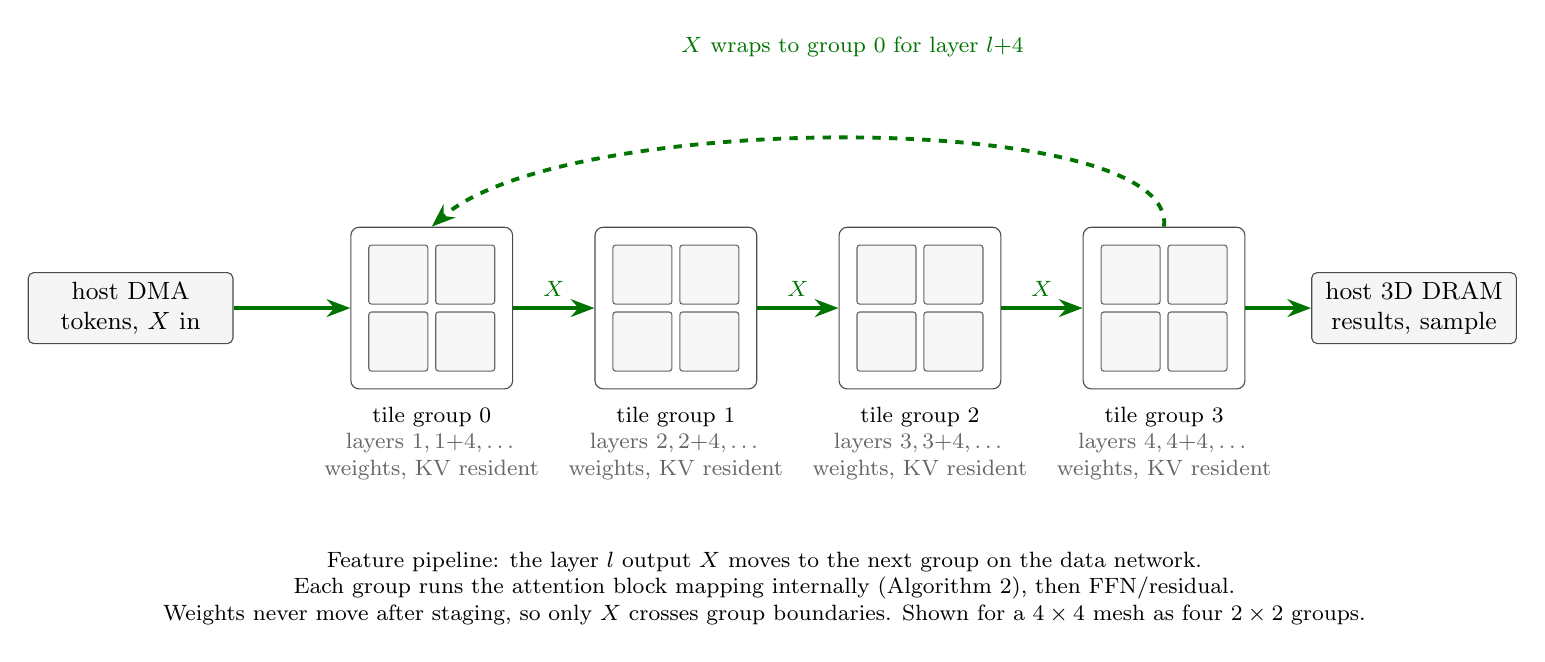
\begin{tikzpicture}[
  tile/.style={draw=black!60, rounded corners=1pt, minimum size=7.5mm,
               fill=gray!6, font=\scriptsize},
  grp/.style={draw=black!70, rounded corners=3pt, inner sep=2.2mm},
  hostbox/.style={draw=black!70, rounded corners=2pt, minimum height=9mm,
                  minimum width=26mm, align=center, fill=gray!8, font=\small},
  xflow/.style={-{Stealth[length=3mm]}, line width=1.4pt, green!45!black},
  note/.style={font=\footnotesize, align=center},
]

% ---- four 2x2 tile groups in a row (one 4x4 mesh, unrolled as stages) ----
\foreach [count=\g from 0] \gx in {0, 3.1, 6.2, 9.3} {
  \foreach \x in {0,1}
    \foreach \y in {0,1}
      \node[tile] (t\g\x\y) at (\gx + 0.85*\x, -0.85*\y) {};
}
\foreach \g in {0,1,2,3} {
  \node[grp, fit=(t\g00)(t\g11)] (g\g) {};
}
\foreach [count=\g from 0] \l in {1, 2, 3, 4} {
  \node[note, anchor=north, yshift=-1mm, align=center] at (g\g.south)
    {tile group \g\\\textcolor{black!60}{layers $\l, \l{+}4, \dots$}\\
     \textcolor{black!60}{weights, KV resident}};
}

% ---- host endpoints ----
\node[hostbox] (hin)  at (-3.4, -0.425) {host DMA\\tokens, $X$ in};
\node[hostbox] (hout) at (12.9, -0.425) {host 3D DRAM\\results, sample};

% ---- activation flow ----
\draw[xflow] (hin.east) -- (g0.west);
\foreach \g [evaluate=\g as \h using int(\g+1)] in {0,1,2} {
  \draw[xflow] (g\g.east) -- (g\h.west)
    node[note, midway, above, green!45!black] {$X$};
}
\draw[xflow] (g3.east) -- (hout.west);

% ---- wrap-around for layer l+4, arcing over the top ----
\draw[xflow, dashed] (g3.north) .. controls (9.9, 2.1) and (2.1, 2.1) .. (g0.north)
  node[note, midway, above, green!45!black, yshift=9mm]
  {$X$ wraps to group 0 for layer $l{+}4$};

% ---- footer ----
\node[note, anchor=north, align=center] at (4.65, -3.4)
  {Feature pipeline: the layer $l$ output $X$ moves to the next group on the data network.\\
   Each group runs the attention block mapping internally (Algorithm 2), then FFN/residual.\\
   Weights never move after staging, so only $X$ crosses group boundaries.
   Shown for a $4 \times 4$ mesh as four $2 \times 2$ groups.};

\end{tikzpicture}
\end{document}
